\documentclass[11p, a4paper, english]{article}
\usepackage[utf8]{inputenc}
\usepackage{babel, lmodern}
\usepackage[text={6in,10in},centering]{geometry}
\usepackage{color}
\usepackage{caption}
\usepackage{xpatch}
\usepackage{graphicx}
\usepackage{subfig}
\usepackage{float}
\usepackage{verbatim}
\usepackage{amsmath}
\usepackage{amssymb}
\usepackage{siunitx}
\usepackage{mathabx}
\usepackage{cleveref}

\title{
\huge{TFY4240 - Computational assignment}
}
\author{Svein Åmdal}
\date{March 2019}


\begin{document}
\maketitle

\section{Setting up the equation}
Given the boundary conditions, we introduce the reduced coordinates $\xi = x/L$ and $\eta = y/L$. We infer that there is no free charge on the square cylinder given in the problem. Therefore, we can find the potential $V$ from solving Laplace's equation

\begin{equation}
\nabla^{2}V(\xi, \eta) = 0,
\end{equation}

for some reduced (i.e. dimensionless) potential $V(\xi, \eta)$. The boundary conditions become

\begin{align}
V(\xi=0, \eta) &= 0 \label{BC1} \\ 
V(\xi=1, \eta) &= 0 \label{BC2} \\
V(\xi, \eta=0) &= 0 \label{BC3} \\
V(\xi, \eta=1) &= V_{0}(\xi). \label{BC4}
\end{align}

There is no dependence on $z$, so we view the problem as two-dimensional. Assuming the potential has a solution of the form $V(\xi, \eta) = X(\xi)Y(\eta)$, we can separate the equation into the form

\begin{equation}
\frac{\partial^{2}_{\xi}X(\xi)}{X(\xi)} + \frac{\partial^{2}_{\eta}Y(\eta)}{Y(\eta)} = 0.
\label{separatedLaplacian}
\end{equation}

Because $\xi$ and $\eta$ are independent, each of the terms in \cref{separatedLaplacian} must individually be constant, say $-k^{2}$ and $k^{2}$, respectively. We may assume $k > 0$. Solving the indivicual equations, we get that

\begin{align}
X(\xi) &= Acos(k\xi)+Bsin(k\xi) \\
Y(\eta) &= Ce^{k\eta}+De^{-k\eta}.
\end{align}

Using \cref{BC1}, we find that $A = 0$. Using \cref{BC3} we get that $C=-D$. Thus $X(\xi) \rightarrow Bsin(k\xi)$ and $Y(\eta) \rightarrow 2Csinh(k\eta)$. Using \cref{BC2}, we find that either $B = 0$, or $k=n\pi$. To ensure the solution is nontrivial, we choose to demand the latter. Finally \cref{BC4} implies that the equation

\begin{equation}
2Bsin(n\pi\xi)Csinh(n\pi) = V_{0}(\xi)
\label{V0BC}
\end{equation}

holds $\forall n \in \mathbb{N}$. The general solution is a linear combination of these. Letting $B \rightarrow B_{n}$ and $C \rightarrow C_{n}$ and combining all constants into $F_{n} = B_{n}C_{n}$, we get

\begin{equation}
V(\xi, \eta) = 2\sum_{n}F_{n}sin(n\pi\xi)sinh(n\pi\eta).
\label{Vtemp}
\end{equation}

Inserting $\eta = 1$ we re-obtain \cref{V0BC}. Mulitplying both sides of \cref{V0BC} with $sin(m\pi\xi)$ and integrating over the interval of $\xi \in (0,1)$, we obtain

\begin{align}
2\int_{0}^{1}d\xi V_{0}(\xi)sin(m\pi\xi) = 2\sum_{n}F_{n}sinh(n\pi)\int_{0}^{1}d\xi sin(n\pi\xi)sin(n\pi\xi) = 2\sum_{n}F_{n}sinh(n\pi)\frac{\delta_{nm}}{2}	\\ 
= F_{m}sinh(m\pi) \implies F_{n} = \frac{1}{sinh(n\pi)}\int_{0}^{1}dqV_{0}(q)sin(n\pi q).
\label{Fn}
\end{align}

Finally, the equation that yields $V$ is then given by

\begin{equation}
V(\xi, \eta) = 2\sum_{n=1}^{\infty}F_{n}sin(n\pi\xi)sinh(n\pi\eta),
\label{V}
\end{equation}

where $F_{n}$ is the $n$-th \textit{Fourier coefficient}, given by \cref{Fn}.


\section{Plots}

\begin{figure}[h!]
\centering
\subfloat[The target function.]{{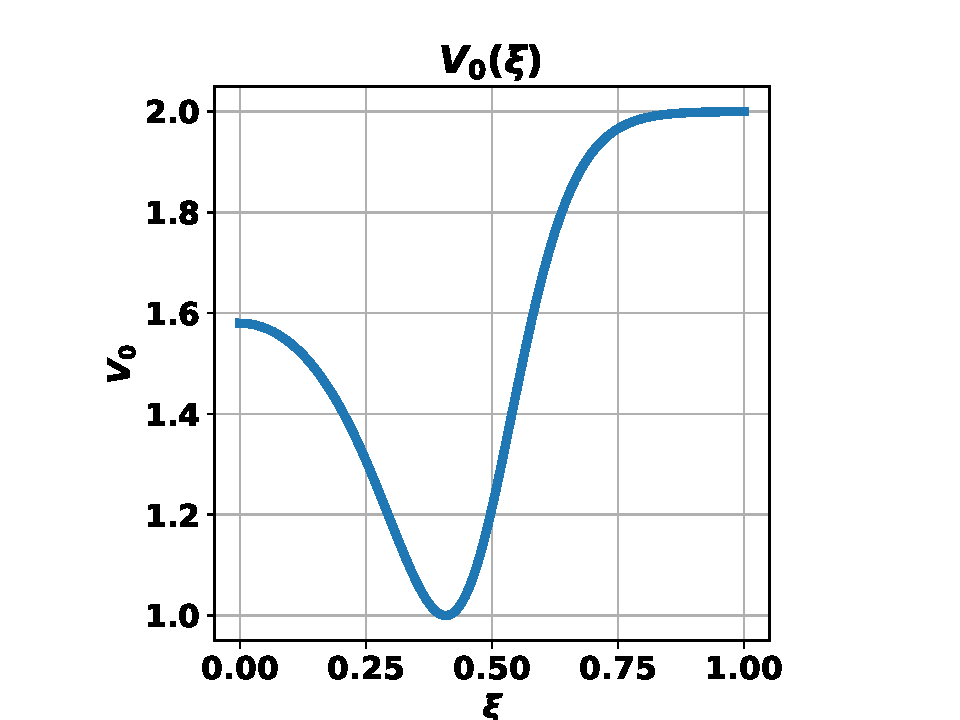
\includegraphics[scale=0.43]{plotV0.pdf}\label{V0}}}
\qquad
\subfloat[Reconstruction of the target function by four Fourier components.]{{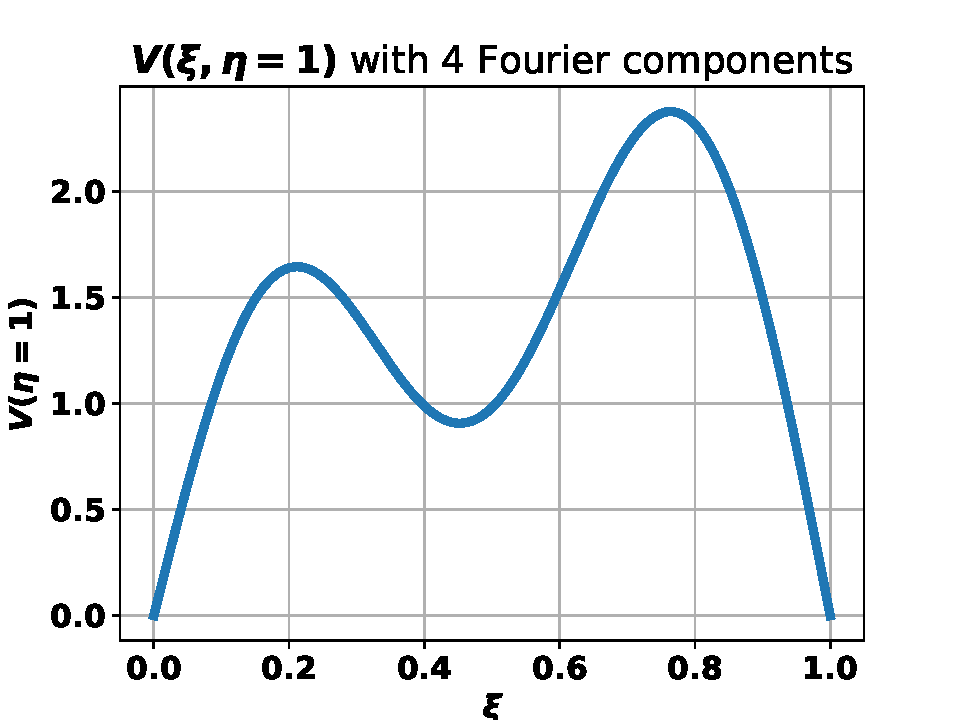
\includegraphics[scale=0.43]{plotVy1.pdf}\label{Vy1}}}
\caption{Plot of $V(\xi, \eta=1)$.}
\label{compFig}
\end{figure}

\begin{figure}[h!]
\centering
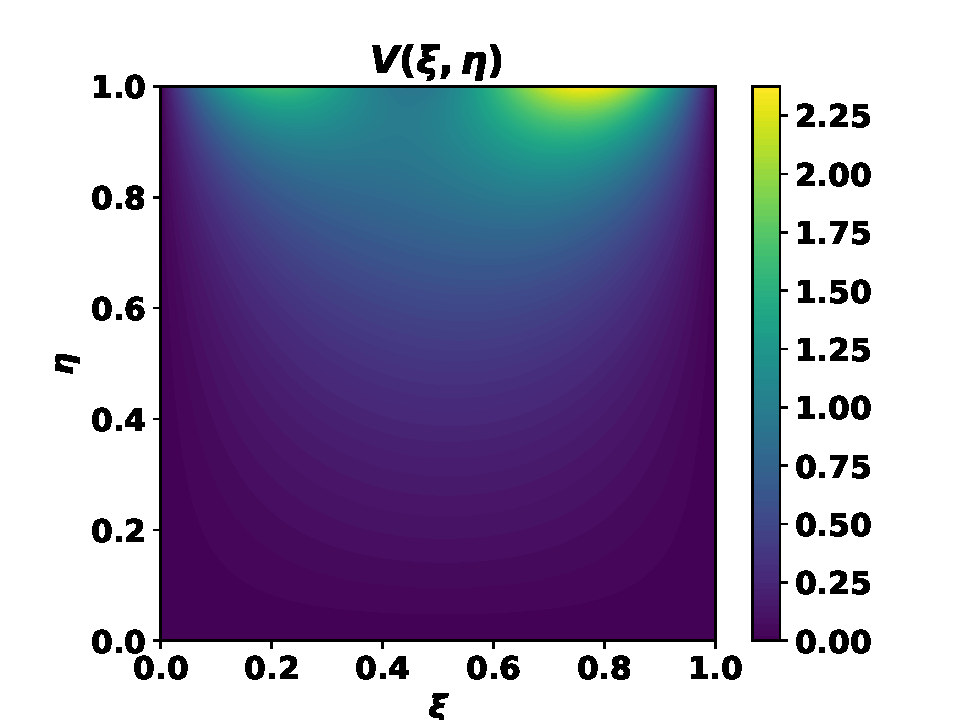
\includegraphics[scale=0.8]{plotVxy.pdf}
\caption{Contour plot of $V(\xi, \eta)$.}
\label{Vxy}
\end{figure}

Comparison between $V_{0}$ and $V(\xi, \eta=1)$ is given in \cref{compFig}. This will be commented further later on. Using $4$ Fourier components, the full solution for $V$ is given in \cref{Vxy}. We use the fact that $\vec{E}(\xi, \eta) = -\nabla_{\xi, \eta} V(\xi, \eta)$ to obtain the solution of $\vec{E}$ (also reduced) in \cref{Exy}.

\begin{figure}[h!]
\begin{center}
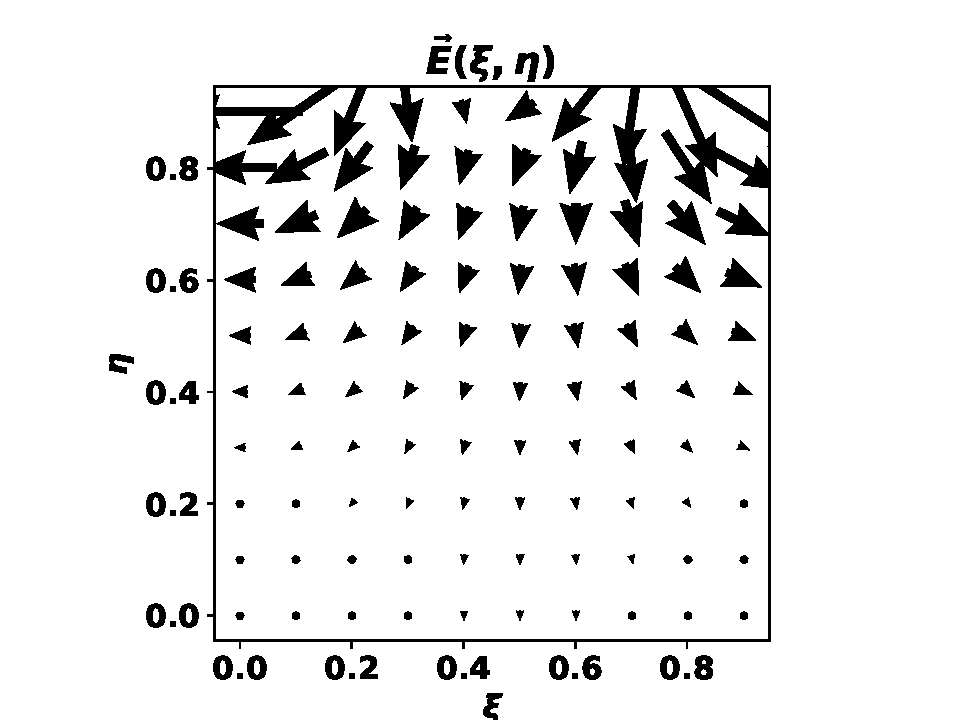
\includegraphics[scale=0.8]{plotExy.pdf}
\caption{Quiver plot of $\vec{E}(\xi, \eta)$.}
\end{center}
\label{Exy}
\end{figure}


\section{Discussion of errors}

We have used the function $V_{0}(\xi) = 1 + tanh^{2}(1 - 6\xi^{2})$. This does not vanish in the end points. The boundary conditions given by \cref{BC1} and \cref{BC2}, \textit{do} however require $V_{0}$ be $0$ here. The function we reconstruct in \cref{Vy1} is in fact discontinious, so any finite Fourier series experiences the Gibbs' phenomena close to the discontinuity. Therefore, we opt to only use terms up to $n=4$. Using higher order terms yields better accuracy close to the boundaries, but also results in some wild behaviour slightly further away. This is shown in \cref{compFourier}. Ultimately, we determined that $n=4$ provided a nice-looking potential, without being computationally intensive. With \cref{compFourier} we also show that increasing $n$ increases the accuracy, in case we want to consider a different $V_{0}$.


\begin{figure}[h!]
\centering
\subfloat[$n$=$12$.]{{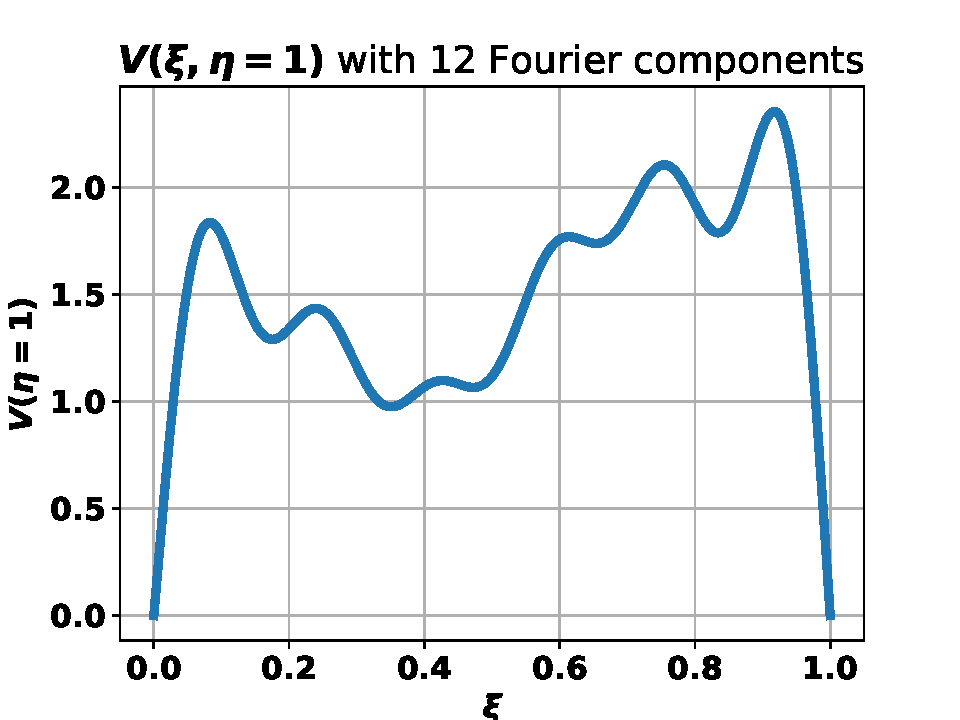
\includegraphics[scale=0.43]{plotVy1_12Fourier.pdf}\label{F12}}}
\qquad
\subfloat[$n$=$100$.]{{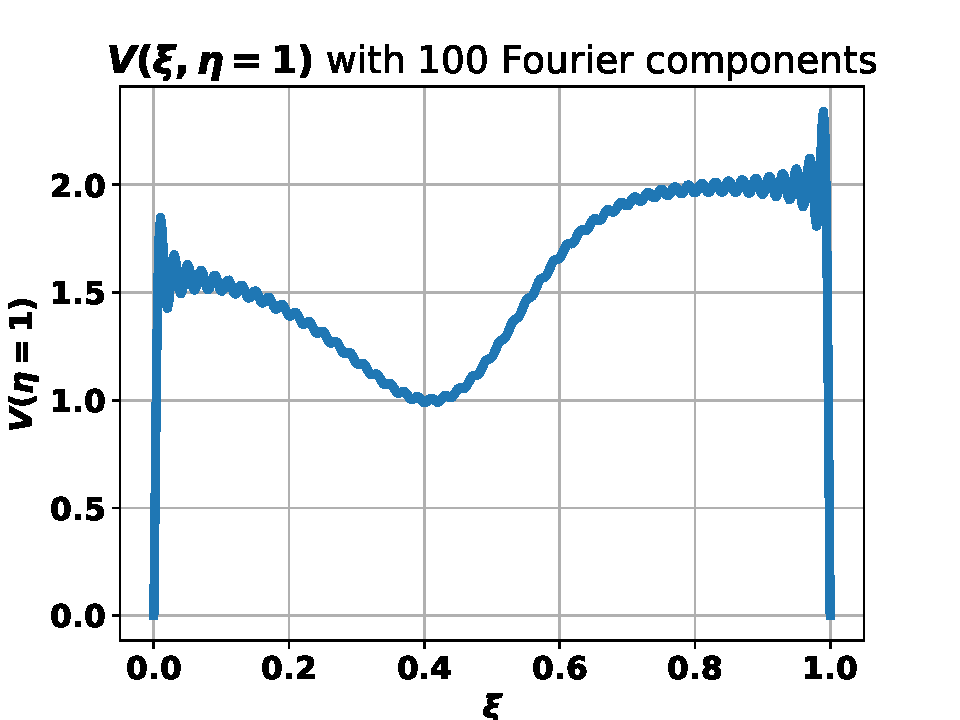
\includegraphics[scale=0.43]{plotVy1_100Fourier.pdf}\label{F100}}}
\caption{Plot of $V(\xi, \eta=1)$ with differing amounts of Fourier components.}
\label{compFourier}
\end{figure}


\end{document}
